\cleardoublepage

\section{The working model}
\label{sec:workframe}

This chapter introduces in the first part the final working model, which was developed to analyse the obtained empirical data. Furthermore, the initial version of it is displayed and the considerations taken are explained. In the second part, another option to visualise the obtained data by using the working model is displayed. This emerged as side product during the development of the main model and can be used as additional perspective in the analysis process.


\subsection{Introduction of the model and considerations}
The need for this model originates, as described before, from the complexity and the amount of qualitative data, which requires structuring in order to be analysed. Figure \ref{fig:final} below depicts the final version of the working model.\\

\begin{figure}[!hbt]
    \captionsetup{font=small}
  \centering
  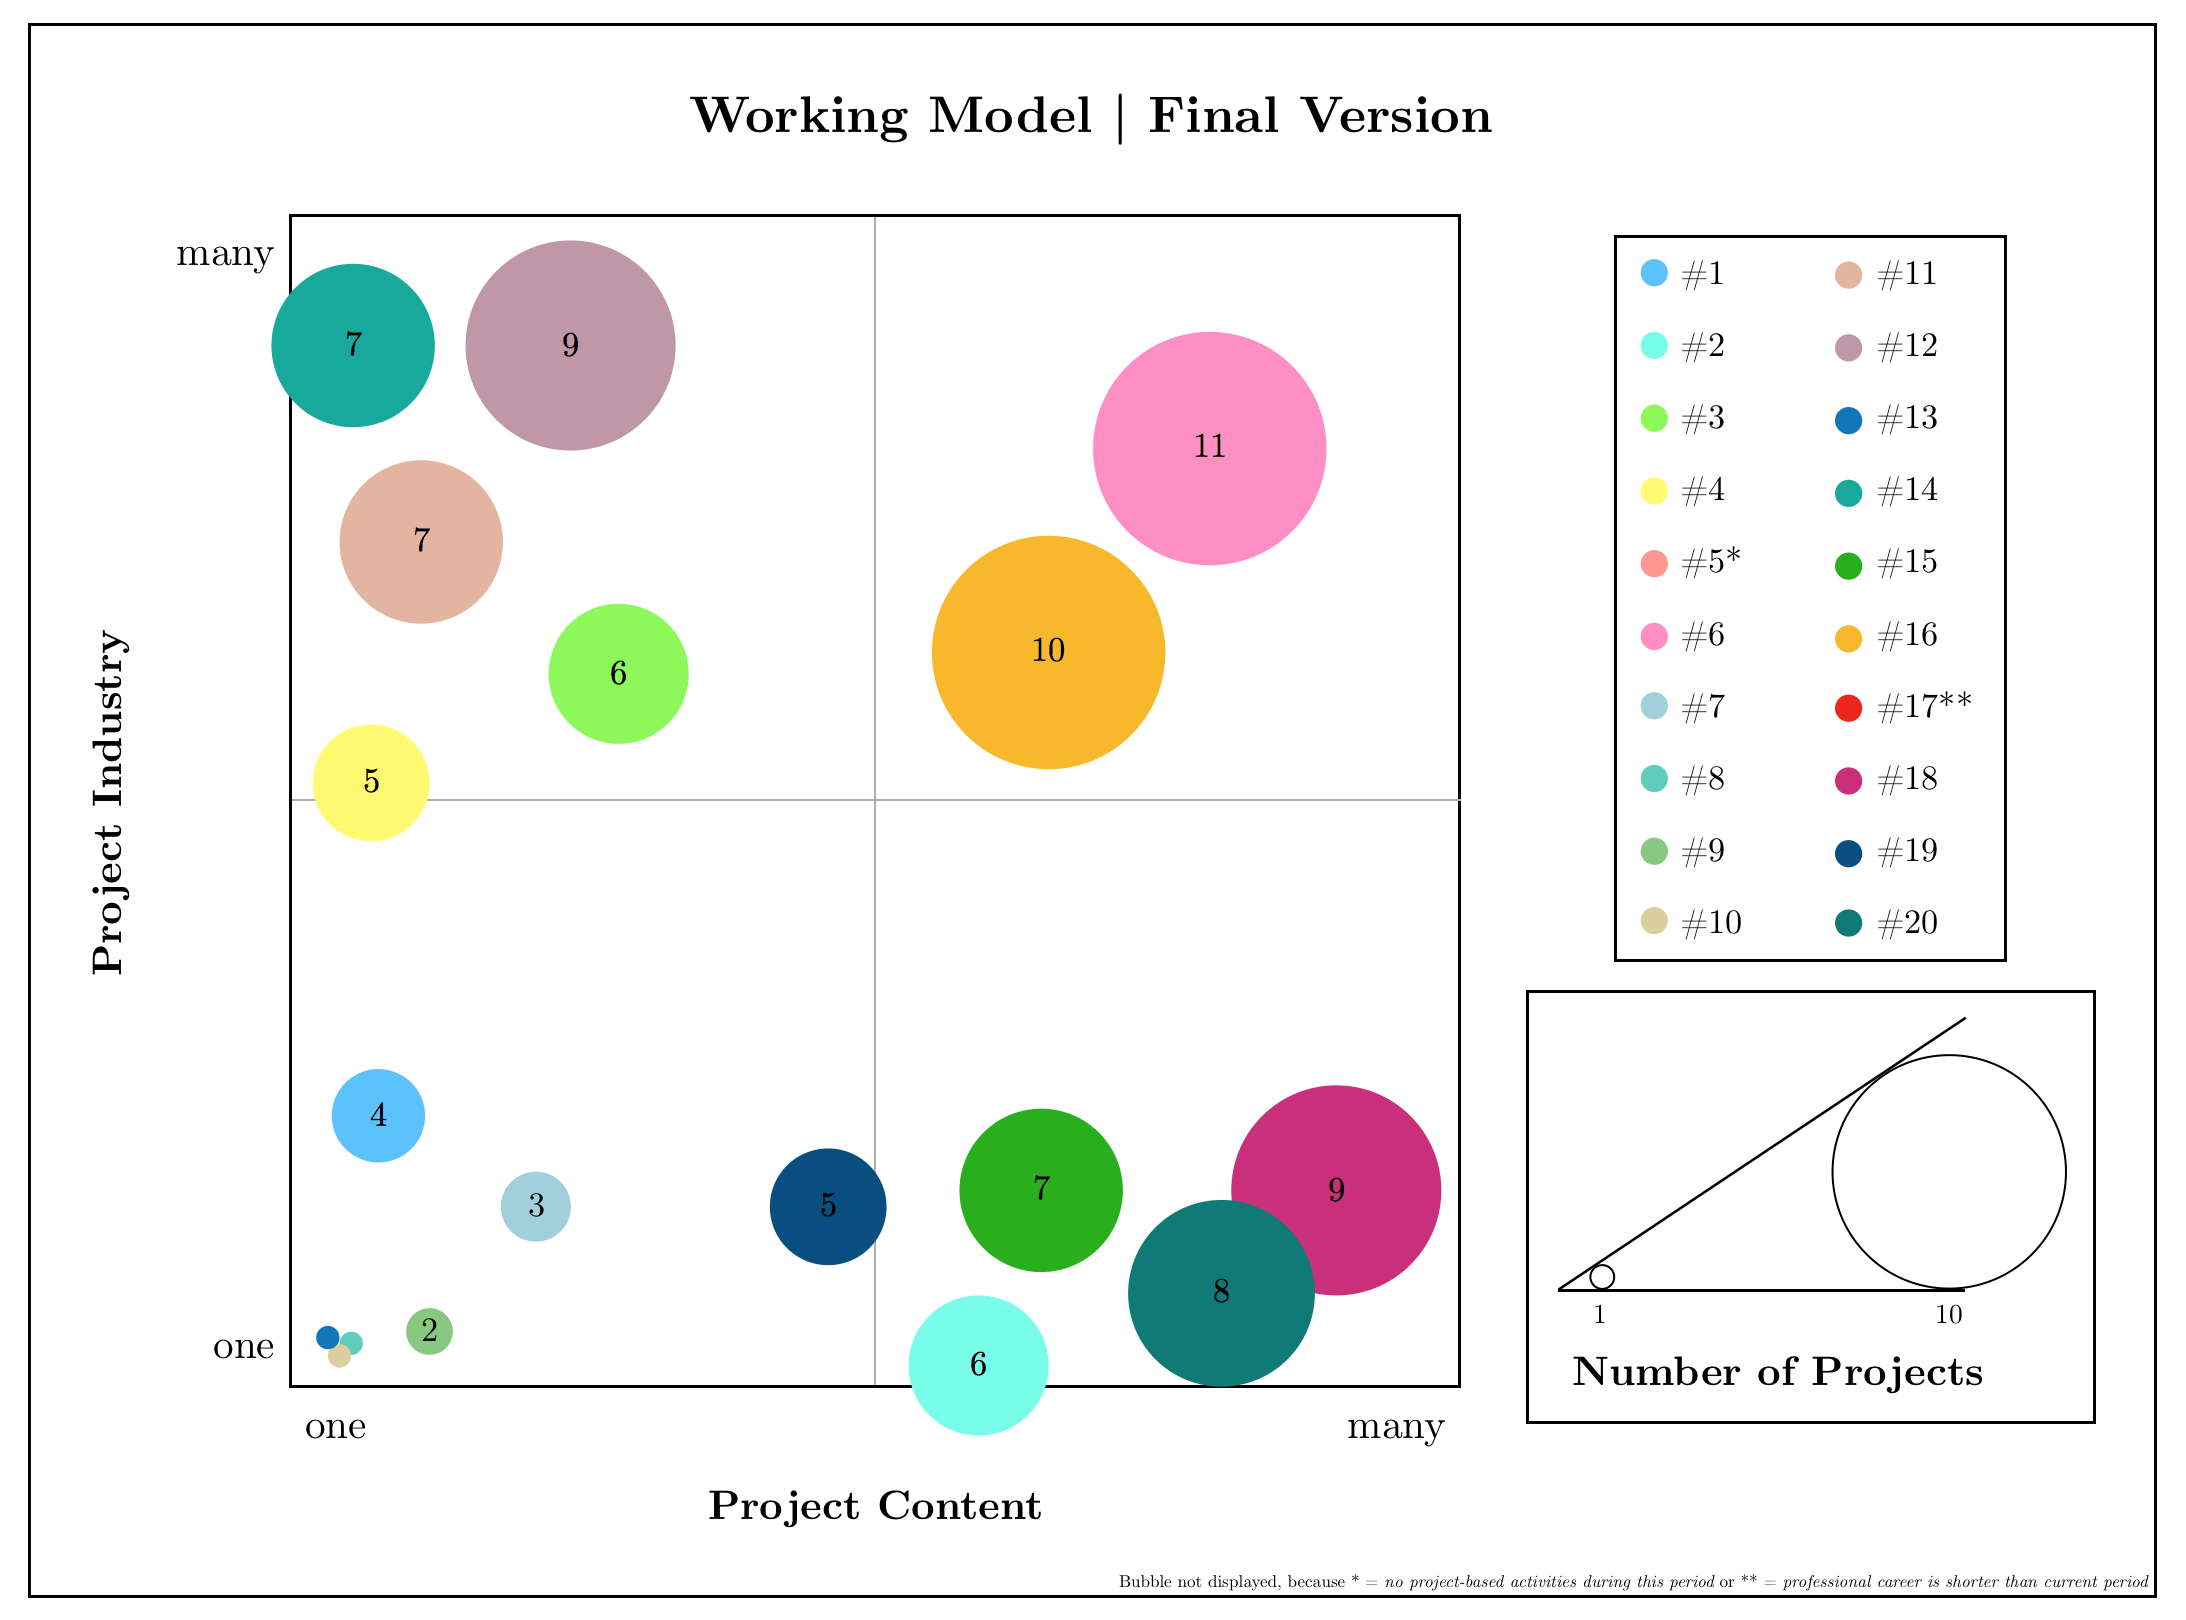
\includegraphics[width=.7\columnwidth]{figures/WM_final.png}
  \caption[The final working model]{The final working model – It comprises three dimensions, project industry ($y$-axis), project content ($x$-axis) and number of projects (bubble diameter and number), as well as a legend which allocates each colour to a candidate's ID (filled with dummy data).}
  \label{fig:final}
\end{figure}

The model exhibits three dimensions of the careers of project professionals. These dimensions are \textit{the number of different project industries}, \textit{the number of different project contents} and \textit{the total number of projects}. The analysis for these three attributes is conducted for periods of five years. This means, if the candidates interviewed have a work experience of 20 years or less, at the end of the analysis you'll have 4 models, one for the first five years, one for the period from the \nth{5} until the \nth{10} year, etc. For these periods the model depicts the attributes for all interviewees, which are differentiated by different colours. Furthermore, there were two reason why a candidate's bubble would not be displayed, the first one being that the candidate did no participate in project-related activities during this period (marked with one asterisk). The second one stands for the absence cause, that the interviewee's career is shorter than the corresponding period (marked with two asterisks). In the following, each of the three named dimensions of the working model are explained in detail.\\

\clearpage

\noindent {\bf Project industry}\\[.1cm]
The categorisation attribute \textit{project industry} is represented by the $y$-axis. Its scale was chosen to be non-numeric (one - many), since the non-numeric scale  allows for easier interpretation of the quadrants. However, the data is filled in based on a numeric scale. This scale was chosen considering the data sets. Therefore, the highest number of different industries within a time span of 5 years was ascertained, which led to a scaling of 1-5. The list of industries that was introduced in Chapter \ref{sec:LiteratureRev:PCategorisation:ByPIndustry} serves thereby as a theoretical structure by which in the analysis process the different industries of the projects in which the candidates worked in are identified and accordingly evaluated. \\

\noindent {\bf Project content}\\[.1cm]
The dimension \textit{project content} is located on the $x$-axis and alike the project industry-attribute its scale is non-numerical. Furthermore, the point's position is, similarly to the $y$-axis scaling, based on a linear scale, which was chosen according to the maximum value to be found in the data sets. As a result, the underlying numerical scale extends from 1 to 5. The differentiation between the various project contents of the project professionals follows the in chapter 2.2.1 introduced list of project contents by \citeA{patzak17}. At this point it is important to mention that the classification attribute 'project content' was not the initial sorting criteria as can be seen in figure \ref{fig:initial} on page \pageref{fig:initial}. Initially, the second dimension was 'project type'. However, the attribute was changed especially due to feedback received by the participants of the focus group workshop, which stated that project type as attribute is too broadly defined and that in the context of project professionals' careers 'project content' makes the most sense. This feedback is also backed by the project management literature, in which project types is used as hypernym for all the project attributes by which projects can be classified. \\

\noindent {\bf Number of projects}\\[.1cm]
In contrast to the other two dimensions the third dimension \textit{number of projects} is not represented by one of the axes, instead it is constituted by the diameter and the number written in the middle of each of the dots (except, if there is only one project). In order to be able to interpret the size of the dots a legend is shown on the right. For reasons of readability the maximum diameter size is limited to a 10 projects bubble and project numbers higher than 10 are only represented by the number in the middle. Furthermore, as can be seen in figure \ref{fig:initial} on page \pageref{fig:initial}, this dimension was not included in the initial model. 
It was added, as early analysis suggested that there may be other potentially relevant dimensions, of which number of projects was chosen as the most promising one. Above all, the third classification attribute was included in order to provide more depth to the model and thereby facilitate the interpretation of the outcomes. \\

\begin{figure}[!hbt]
    \captionsetup{font=small}
  \centering
  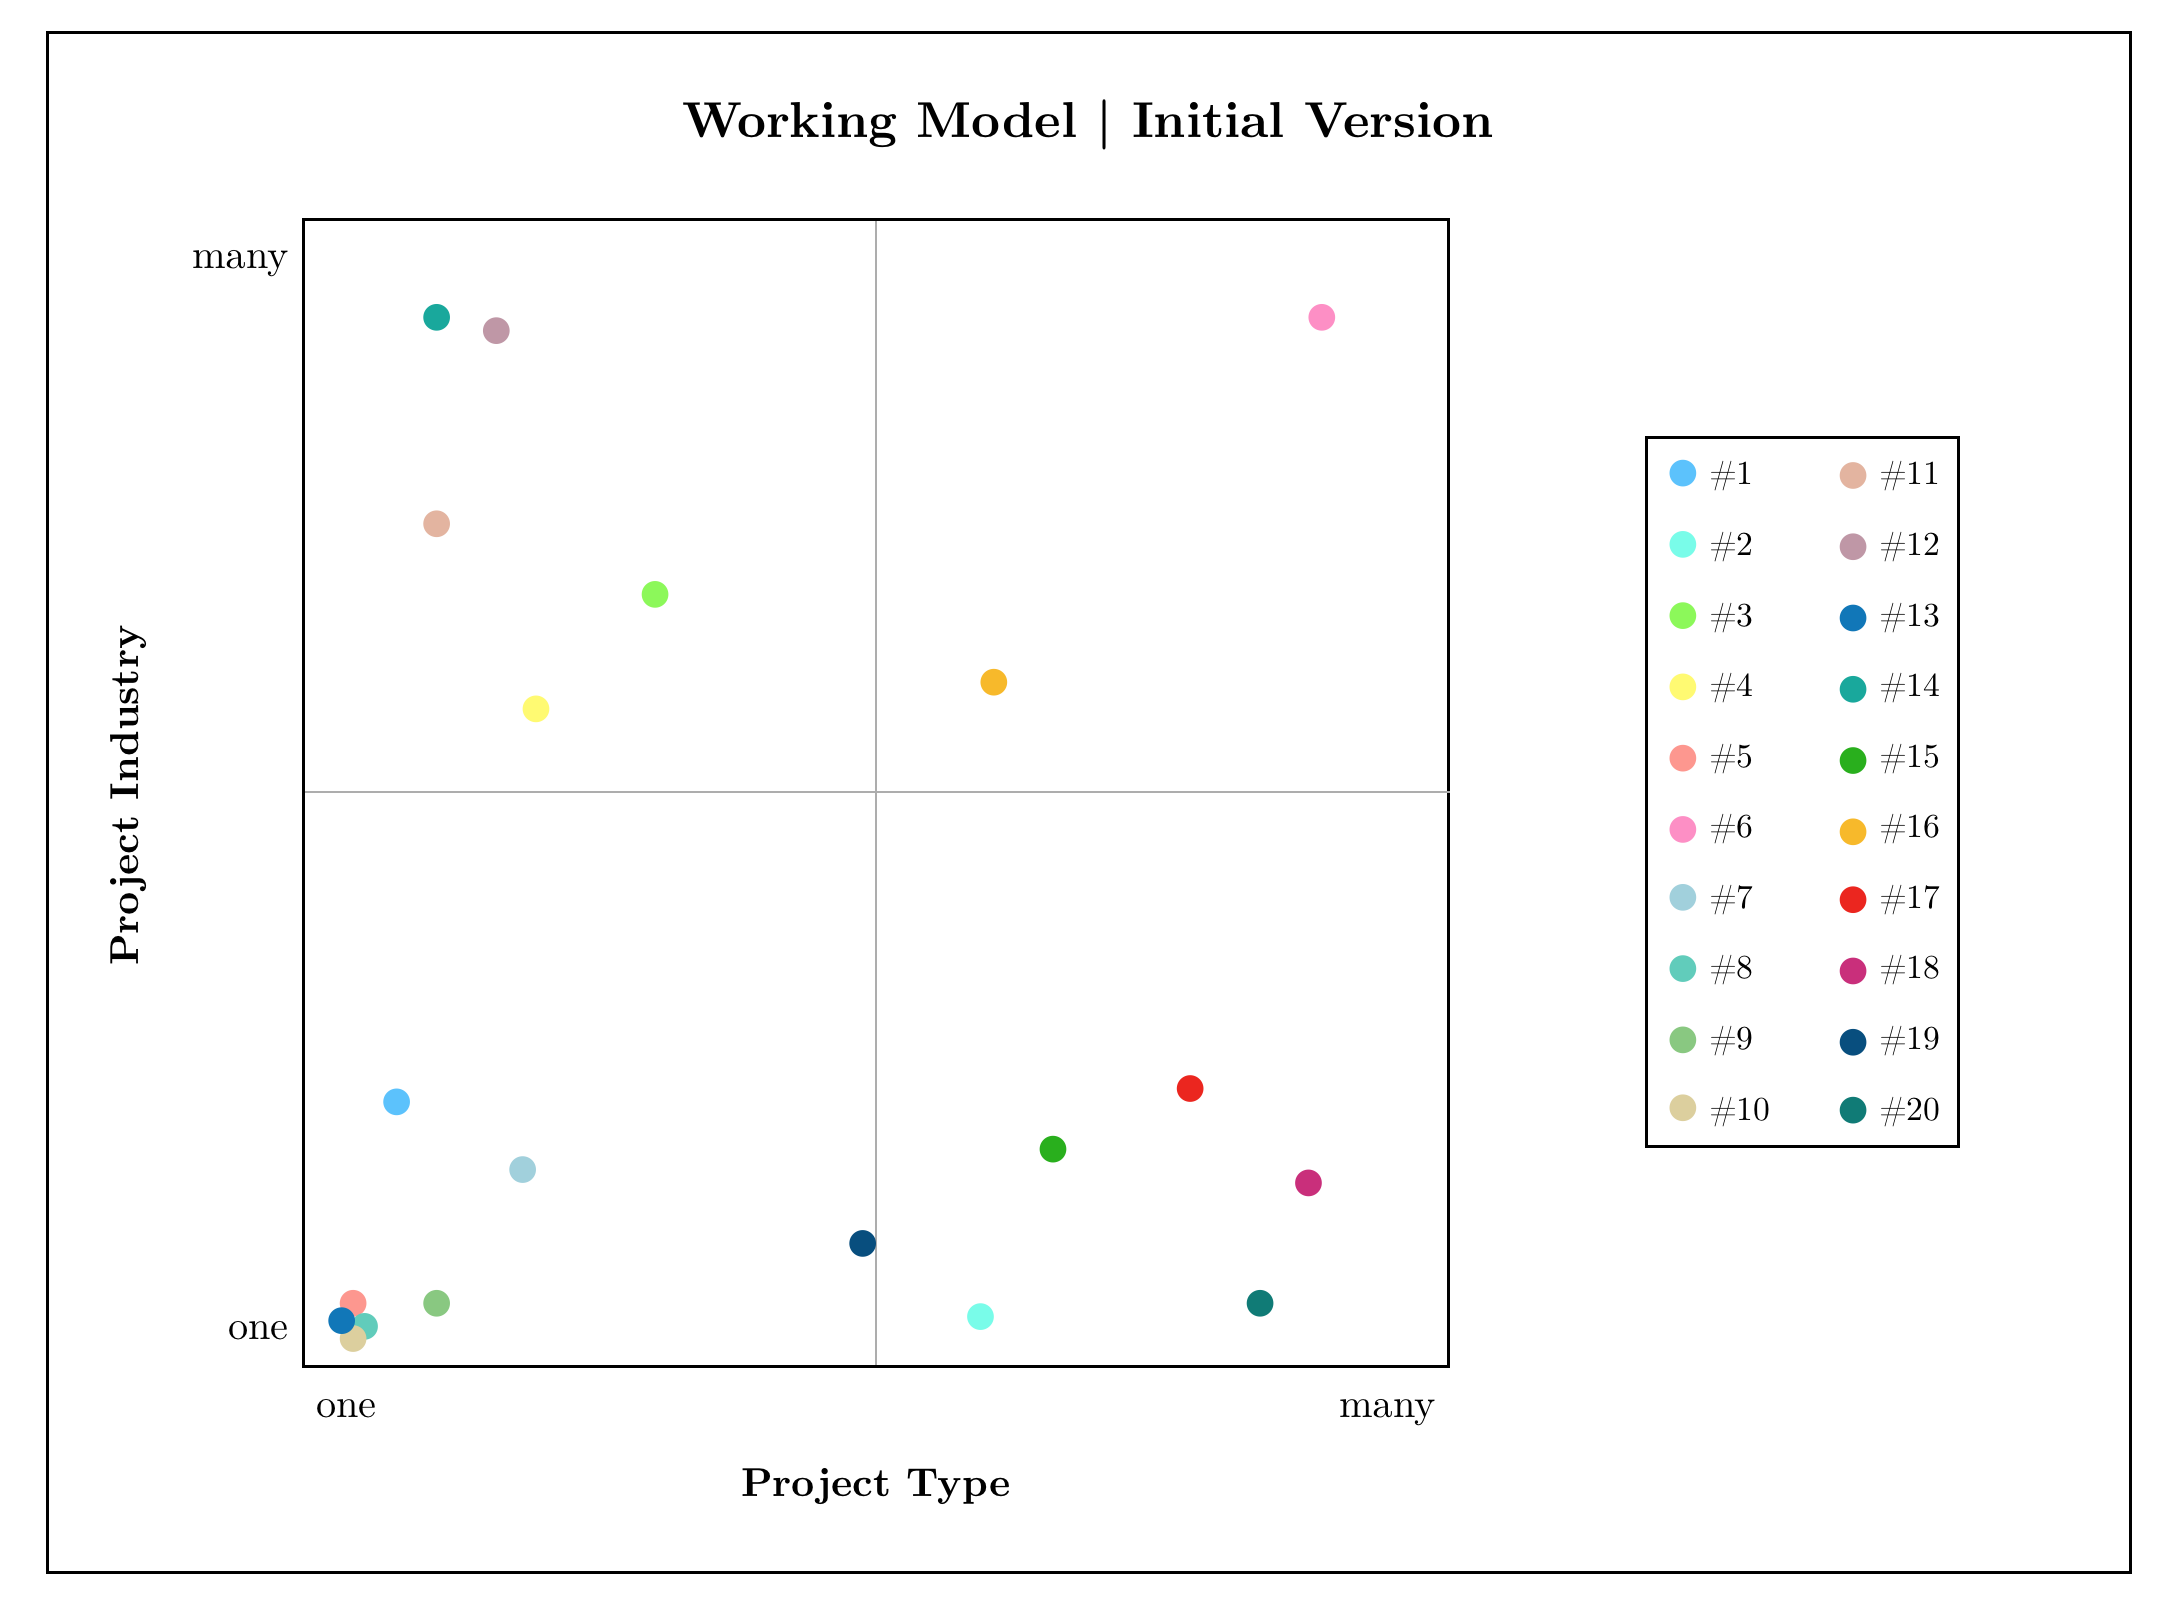
\includegraphics[width=.45\columnwidth]{figures/WM_Initial.png}
  \caption[The initial working model]{The initial working model (filled with dummy data).}
  \label{fig:initial}
\end{figure}

%\clearpage


\subsection{An alternate variant – The career movement model}
\label{sec:cmm}
The alternative variant of the final working model, \textit{The career movement model}, which is shown below in figure \ref{fig:alternate}, was included in this bachelor thesis, since it provides an interesting, different viewpoint on the research data. It includes, in contrast to the final model only the two main dimensions on the axes. Instead of the third dimension, it shows for each candidate, his/her position in the map during each of the five-year periods since the start of his/her professional career. In other words, it makes movements of a project professional during his/her career in respect to project content and industry visible and is therefore named career movement model. In detail, each of the dots represents one of the periods and the number indicates which it was (1: 0-\nth{5} year, 2: \nth{5}-\nth{10} year, etc.). As a result, it enables the researcher, on the one hand, to compile the stages of the project professionals' career to see them all in one model, in contrast to the final model. Furthermore, it uncovers periods in a project professional's career in which he/she did not work in projects at all. This is visualised by a missing dot and the corresponding number, as can be seen for explanatory purposes in figure \ref{fig:alternate} where in candidate 3's career path the \nth{3} stage is missing. In order to make it visible if a project professional did not do any projects at all in the last periods of his/her career, in this case one grey bubble(s) with the corresponding number for each period is added to the last project bubble. Above all, it facilitates the comparison during the analysis process of the careers of project professionals among themselves and in between different industries, as well as regarding other candidate specific criteria. Thereby, this variant contributes to one of the core research questions of finding patterns in project professional's careers. \\


\begin{figure}[!hbt]
    \captionsetup{font=small}
  \centering
  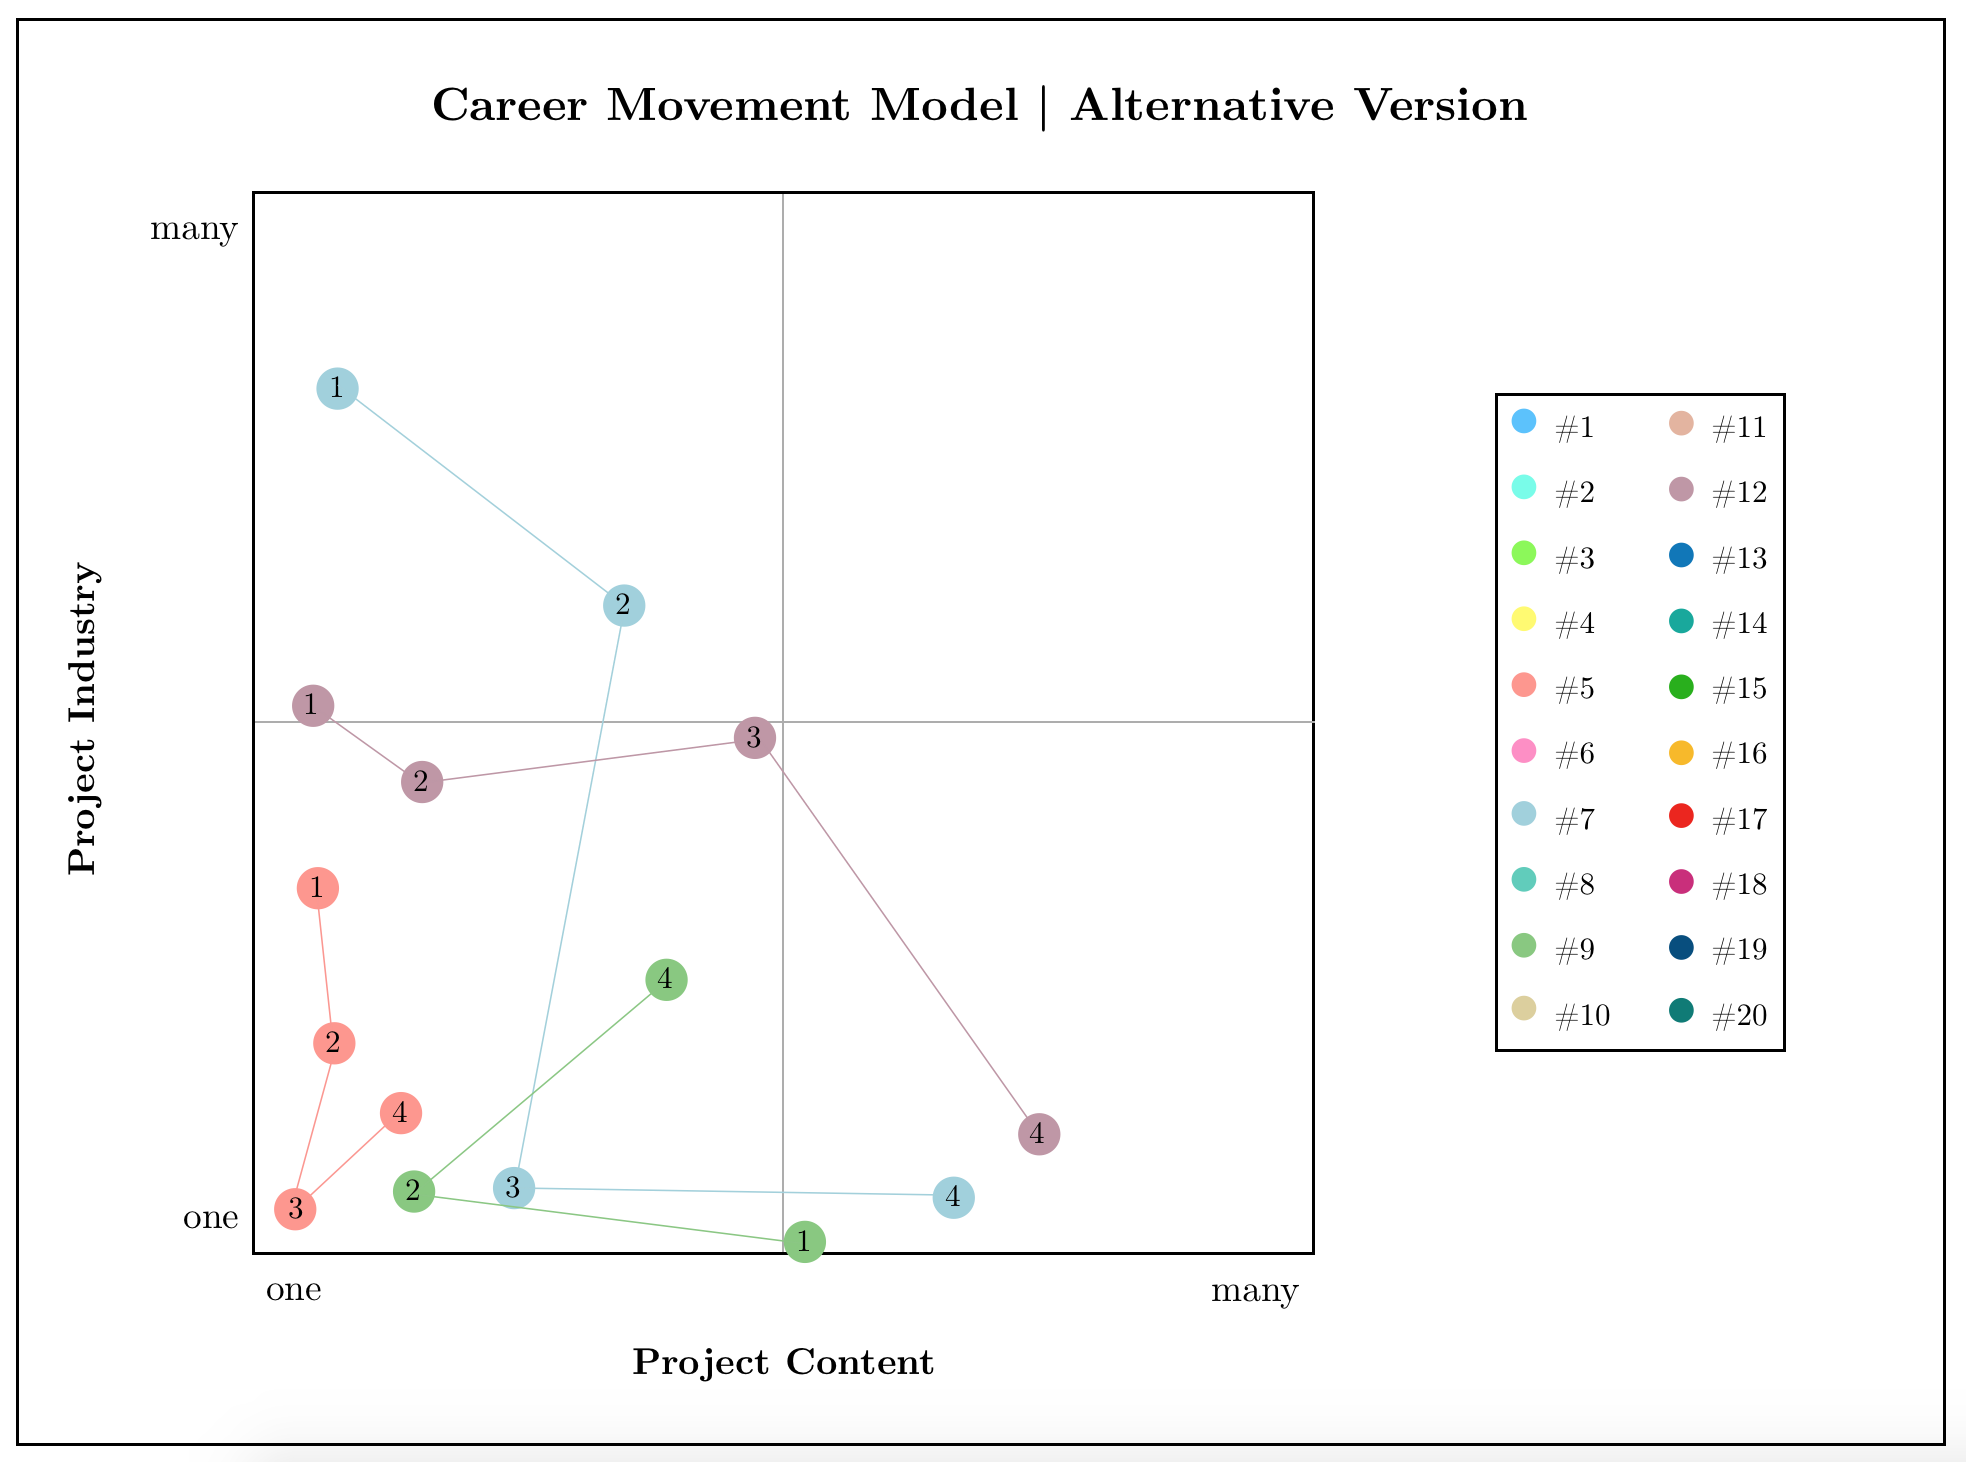
\includegraphics[width=.7\columnwidth]{figures/WM_alternate.png}
  \caption[The career movement model]{The career movement model – An alternative variant of the final working model. It comprises the same axes dimensions, project industry ($y$-axis) and project content ($x$-axes), but instead of the third dimension, it shows the position for each of the career periods, indicated by the number in the bubble (filled with dummy data).}
  \label{fig:alternate}
\end{figure}

